\documentclass[12pt]{scrartcl}
 \usepackage{fancyhdr, graphicx}
 \usepackage[utf8]{inputenc} 
 \usepackage[german]{babel}
 \usepackage[scaled=0.92]{helvet}
 \usepackage{enumitem}
 \usepackage{parskip}
 \usepackage[utf8]{inputenc}
 \usepackage{listingsutf8}
 \usepackage{lastpage} % for getting last page number
 \renewcommand{\familydefault}{\sfdefault}
 
 % Code listenings
\usepackage{color}
\usepackage{xcolor}
\usepackage{caption}
\DeclareCaptionFont{white}{\color{white}}
\DeclareCaptionFormat{listing}{\colorbox{gray}{\parbox{\textwidth}{#1#2#3}}}
\captionsetup[lstlisting]{format=listing,labelfont=white,textfont=white}
\lstset{literate=%
    {Ö}{{\"O}}1
    {Ä}{{\"A}}1
    {Ü}{{\"U}}1
    {ß}{{\ss}}1
    {ü}{{\"u}}1
    {ä}{{\"a}}1
    {ö}{{\"o}}1
    {á}{{\'a}}1
    {í}{{\'i}}1
    {é}{{\'e}}1
    {ý}{{\'y}}1
    {ú}{{\'u}}1
    {ó}{{\'o}}1
    {é}{{\'{e}}}1
    {è}{{\`{e}}}1
    {È}{{\`{E}}}1
    {ê}{{\^{e}}}1
    {ë}{{\¨{e}}}1
    {É}{{\'{E}}}1
    {Ê}{{\^{E}}}1
    {û}{{\^{u}}}1
    {ù}{{\`{u}}}1
    {â}{{\^{a}}}1
    {à}{{\`{a}}}1
    {á}{{\'{a}}}1
    {ã}{{\~{a}}}1
    {Á}{{\'{A}}}1
    {Â}{{\^{A}}}1
    {Ã}{{\~{A}}}1
    {ç}{{\c{c}}}1
    {Ç}{{\c{C}}}1
    {õ}{{\~{o}}}1
    {ó}{{\'{o}}}1
    {ô}{{\^{o}}}1
    {Õ}{{\~{O}}}1
    {Ó}{{\'{O}}}1
    {Ô}{{\^{O}}}1
    {î}{{\^{i}}}1
    {Î}{{\^{I}}}1
    {í}{{\'{i}}}1
    {Í}{{\~{Í}}}1
    {ě}{{\v{e}}}1
    {š}{{\v{s}}}1
    {č}{{\v{c}}}1
    {ř}{{\v{r}}}1
    {ž}{{\v{z}}}1
    {ď}{{\v{d}}}1
    {ť}{{\v{t}}}1
    {ň}{{\v{n}}}1                
    {ů}{{\r{u}}}1
    {Á}{{\'A}}1
    {Í}{{\'I}}1
    {É}{{\'E}}1
    {Ý}{{\'Y}}1
    {Ú}{{\'U}}1
    {Ó}{{\'O}}1
    {Ě}{{\v{E}}}1
    {Š}{{\v{S}}}1
    {Č}{{\v{C}}}1
    {Ř}{{\v{R}}}1
    {Ž}{{\v{Z}}}1
    {Ď}{{\v{D}}}1
    {Ť}{{\v{T}}}1
    {Ň}{{\v{N}}}1                
    {Ů}{{\r{U}}}1
    {~}{{\textasciitilde}}1
}

\lstdefinestyle{XMLStyle}{
morekeywords={error-page,error-code,location},
 language=xml,
 basicstyle=\footnotesize\ttfamily, % Standardschrift
 numbers=left, % Ort der Zeilennummern
 numberstyle=\tiny, % Stil der Zeilennummern
 stepnumber=5, % Abstand zwischen den Zeilennummern
 numbersep=5pt, % Abstand der Nummern zum Text
 tabsize=2, % Groesse von Tabs
 extendedchars=true, %
 breaklines=true, % Zeilen werden Umgebrochen
 frame=b,
 %commentstyle=\itshape\color{LightLime}, Was isch das? O_o
 %keywordstyle=\bfseries\color{DarkPurple}, und das O_o
 basicstyle=\footnotesize\ttfamily,
 stringstyle=\color[RGB]{42,0,255}\ttfamily, % Farbe der String
 keywordstyle=\color[RGB]{127,0,85}\ttfamily, % Farbe der Keywords
 commentstyle=\color[RGB]{63,127,95}\ttfamily, % Farbe des Kommentars
 showspaces=false, % Leerzeichen anzeigen ?
 showtabs=false, % Tabs anzeigen ?
 xleftmargin=17pt,
 framexleftmargin=17pt,
 framexrightmargin=5pt,
 framexbottommargin=4pt,
 showstringspaces=false % Leerzeichen in Strings anzeigen ?
}

\lstdefinestyle{SQLStyle}{
morekeywords={CREATE TABLE IF NOT EXISTS, COLLATE, NOT NULL, ENGINE, PRIMARY KEY,DEFAULT CHARSET},
 language=sql,
 basicstyle=\footnotesize\ttfamily, % Standardschrift
 numbers=left, % Ort der Zeilennummern
 numberstyle=\tiny, % Stil der Zeilennummern
 stepnumber=5, % Abstand zwischen den Zeilennummern
 numbersep=5pt, % Abstand der Nummern zum Text
 tabsize=2, % Groesse von Tabs
 extendedchars=true, %
 breaklines=true, % Zeilen werden Umgebrochen
 frame=b,
 %commentstyle=\itshape\color{LightLime}, Was isch das? O_o
 %keywordstyle=\bfseries\color{DarkPurple}, und das O_o
 basicstyle=\footnotesize\ttfamily,
 stringstyle=\color[RGB]{42,0,255}\ttfamily, % Farbe der String
 keywordstyle=\color[RGB]{127,0,85}\ttfamily, % Farbe der Keywords
 commentstyle=\color[RGB]{63,127,95}\ttfamily, % Farbe des Kommentars
 showspaces=false, % Leerzeichen anzeigen ?
 showtabs=false, % Tabs anzeigen ?
 xleftmargin=17pt,
 framexleftmargin=17pt,
 framexrightmargin=5pt,
 framexbottommargin=4pt,
 showstringspaces=false % Leerzeichen in Strings anzeigen ?
}

\lstdefinestyle{JavaStyle}{
 language=java,
 basicstyle=\footnotesize\ttfamily, % Standardschrift
 numbers=left, % Ort der Zeilennummern
 numberstyle=\tiny, % Stil der Zeilennummern
 stepnumber=5, % Abstand zwischen den Zeilennummern
 numbersep=5pt, % Abstand der Nummern zum Text
 tabsize=2, % Groesse von Tabs
 extendedchars=true, %
 breaklines=true, % Zeilen werden Umgebrochen
 frame=b,
 %commentstyle=\itshape\color{LightLime}, Was isch das? O_o
 %keywordstyle=\bfseries\color{DarkPurple}, und das O_o
 basicstyle=\footnotesize\ttfamily,
 stringstyle=\color[RGB]{42,0,255}\ttfamily, % Farbe der String
 keywordstyle=\color[RGB]{127,0,85}\ttfamily, % Farbe der Keywords
 commentstyle=\color[RGB]{63,127,95}\ttfamily, % Farbe des Kommentars
 showspaces=false, % Leerzeichen anzeigen ?
 showtabs=false, % Tabs anzeigen ?
 xleftmargin=17pt,
 framexleftmargin=17pt,
 framexrightmargin=5pt,
 framexbottommargin=4pt,
 showstringspaces=false % Leerzeichen in Strings anzeigen ?
}
 
 \captionsetup[lstlisting]{format=listing,labelfont=white,textfont=white}
 \fancypagestyle{firststyle}{ %Style of the first page
 \fancyhf{}
 \fancyheadoffset[L]{0.6cm}
 \lhead{
 
\includegraphics[scale=0.8]{./fhnw_ht_e_10mm.jpg}}
 \renewcommand{\headrulewidth}{0pt}
 \lfoot{APSI Lab 2}
 \rfoot{Daniel Gürber, Stefan Eggenschwiler}
}

\fancypagestyle{documentstyle}{ %Style of the rest of the document
 \fancyhf{}
 \fancyheadoffset[L]{0.6cm}
\lhead{
 
\includegraphics[scale=0.8]{./fhnw_ht_e_10mm.jpg}}
 \renewcommand{\headrulewidth}{0pt}
 \lfoot{\thepage\ / \pageref{LastPage}}
}

\pagestyle{firststyle} %different look of first page
 
\author{Stefan Eggenschwiler \& Daniel Gürber}
\title{ %Titel
Application Security
\\Lab 2
\vspace{0.2cm}
}

 \begin{document}
 \maketitle
 \thispagestyle{firststyle}
 \pagestyle{firststyle}
 \begin{abstract}
 \begin{center}
 \end{center}
 \vspace{0.5cm}
\hrulefill
\end{abstract}

 \pagestyle{documentstyle}
 \tableofcontents
 \pagebreak
\section{Aufgabenstellung}
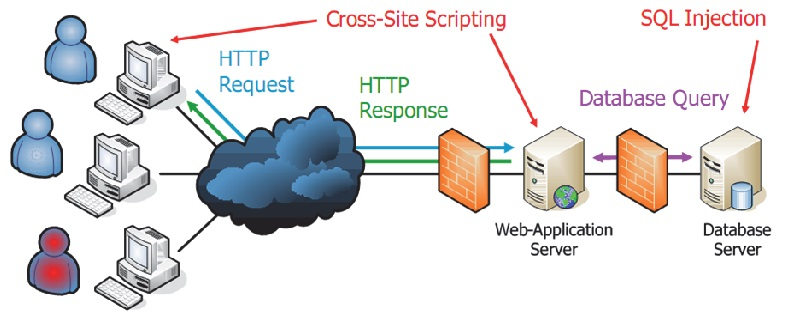
\includegraphics[scale=0.5]{./aufgabenstellung.jpg}

\section{Softwareaufbau}
Die Applikation wurde so programmiert, dass sie auf einem Tomcat lauffähig ist und dabei auf eine MySql Datenbank zugreift. Die Applikation ist aufgeteils in Servlets, Controller, Model, JSP-Pages und MailService.
\subsection{Servlets}
Die Servlets reagieren jeweils auf ein URL-Pattern und leiten die Anfragen zu den entsprechenden Methoden auf dem Controller.
\begin{itemize}
\item IndexServlet: Leitet GET-Anfragen auf /Index auf den Controller weiter, um die Startseite anzuzeigen.
\item LoginServlet: Leitet GET- und POST-Anfragen auf /Login auf den Controller weiter um die Login Seite anzuzeigen bzw. die Login Anfrage zu bearbeiten.
\item OverviewServlet: Leitet GET- und POST-Anfragen auf /Overview auf den Controller weiter um die Übersichts Seite anzuzeigen bzw. die Passwortänderungs Anfrage zu bearbeiten.
\item OverviewServlet: Leitet GET- und POST-Anfragen auf /Register auf den Controller weiter um die Registrierungs Seite anzuzeigen bzw. die Registrierungs Anfrage zu bearbeiten.
\end{itemize}
\subsection{Controller}
Die Controller-Klasse kann nicht instanziert werden, da der Konstruktor auf private gesetzt ist, sie bietet statische Methoden an, um eingehende HttpServletRequests zu behandeln. Die einzelnen Methoden analysieren  und validieren den Request, rufen entsprechende Methoden auf dem Model auf um Daten zu laden oder zu ändern und zeigen als HttpServletResponse JSP-Pages als View an oder leiten den Benutzer auf eine andere URL um.
\subsection{Model}
Die Model-Klassen enthalten alle Logik, um das Datenmodel auszulesen, zu validieren und zu ändern.
\subsubsection{Comapny}
Die Klasse Company hat zwei Anwendungen:
Einerseits kann sie mit Feldwerten instanziert werden und diese Werte mit Instanzmethoden zu Validieren und in die Datenbank zu speichern, alle Felder sind final.
Andererseits bietet die Klasse auch statische Methoden um Daten zu laden, zu validieren und zu ändern, diese werden verwendet um dem Login durchzuführen, das Passwort zu ändern oder um ein Zitat zu laden.
\subsubsection{ConnectionHandler}
Diese Klasse kann nicht instanziert werden, sie enthält eine statische Methode um eine Verbindung auf die Datenbank zu erhalten.
\subsubsection{Utils}
Diese Klasse kann nicht instanziert werden, sie enthält eine statische Methode um eine einen String für Html sicher zu parsen, und würde um weitere allgemeine Methoden erweitert werden.
\subsection{JSP-Files}
Die JSP-Files stellen Templates dar, die mit Informationen vom Controller gefüllt als Html an den Browser gesendet werden.
\subsection{MailService}
Diese Klasse kann nicht instanziert werden, sie bietet eine statische Methode um ein E-Mail für die Registrierung einer Firma zu senden.
\section{Datenbank}
Die Datenbank läuft unter einem MySql-Server.
\subsection{Aufbau}
Die einzige Tabelle auf der Datenbank ist company, da der username für das Login eindeutig sein muss, ist er als Primärschlüssel geeignet und definiert.
\lstinputlisting[caption=Database Script,style=SQLStyle]{data_structure.sql}
\subsection{Sicherheit}
Für den Zugriff über die Applikation wurde ein user apsilab02 erstellt, dessen Rechte auf CRUD-Operationen auf der Tabelle company limitiert sind. Für den Root-User wird ein Passwort festgelegt und die Datenbank wird so eingestellt, das nur von localhost darauf zugegriffen werden kann (oder als IP-Limitation wenn die Applikation nicht auf dem selben Server ausgeführt wird).
\section{Validierung}
Im folgenden gehen wir auf die Validierung der Inputdaten ein. Angegeben werden jeweils die Voraussetzungen aus der Aufgabenstellung und wie wir diese implementiert haben.

\subsection{Firmenname}
Nur Gross- und Klein-Buchstaben und Leerzeichen (max. 20).
\lstinputlisting[caption=Validierung Firmenname,style=JavaStyle]{firma.java}

\subsection{Strasse \& Strassennummer}
Gross- und Klein-Buchstaben, Zahlen, Punkt, Bindestrich, Leerzeichen.
\lstinputlisting[caption=Validierung Adresse,style=JavaStyle]{address.java}

\subsection{Postleitzahl}
Nur Zahlen, richtige PLZ für die Schweiz, nachkontrolliert mit einem Web-Dienst wie z. B.: http://www.postleitzahlen.ch.
\lstinputlisting[caption=Validierung PLZ,style=JavaStyle]{zip.java}

\subsection{Stadt}
Erlaubte Zeichen: Gross- und Klein-Buchstaben, Punkt, Bindestrich, Leerzeichen.
\lstinputlisting[caption=Validierung Stadt,style=JavaStyle]{town.java}

\subsection{E-Mail Adresse}
Sie senden aber erst, wenn Sie sicher sind, dass die
Email-Adresse auch existiert (no bouncing).
\lstinputlisting[caption=Validierung E-Mail,style=JavaStyle]{mail.java}

\subsection{Benutzername}
min. 4 Zeichen, max. 64 Zeichen; Erlaubte Zeichen:
Zahlen, Gross- und Klein-Buchstaben mit Umlauten, Punkte, Bindestriche, Unterstriche.

\subsection{Passwort}
min. 8 Zeichen, max. 64 Zeichen; Erlaubte Zeichen: Zahlen, Gross- und Klein-Buchstaben mit Umlauten, Punkten, Bindestrichen, Unterstrichen.
\lstinputlisting[caption=Validierung Passwort,style=JavaStyle]{password.java}

\section{Sicherheit}
\subsection{SQL-Injection}
Die Validierung der Werte vor dem ausführen der Speicher-Funktion sollte schon verhindern, dass gefährliche Zeichen in den Feldwerten vorhanden sind. Trotz dieser Absicherung werden die SQL-Statements fest mit Platzhaltern als PreparedStatement definiert und die Feldwerte werden darüber gesetzt, wodurch sie nur als Daten und nicht als Befehle interpretiert werden können.
\lstinputlisting[caption=PreparedStatement,style=JavaStyle]{sql.java}
\subsection{Cross-site Scripting}
Um Cross-site Scripting zu verhindern werden in den JSP-Files nur dynamische Inhalte dargestellt, welche vom Controller gesetzt wurden und keine Daten aus den Request-Parameter. Der Controller ruft für alle Ausgaben, welche nicht fest im Programm definiert sind, an die JSP-Files zuerst die Funktion encodeHtml auf, welche alle potentiell gefährlichen Zeichen durch Html-Platzhalter ersetzt.
\lstinputlisting[caption=encodeHtml,style=JavaStyle]{encodeHtml.java}
\subsection{Error Handling}
Damit keine internen Informationen über die Implementierung nach aussen dringen, wurden im web.xml zwei Seiten definiert, welche bei Fehlern angezeigt werden. 404.jsp wird dem User angezeigt, wenn unter der eingegebenen URL keine Ressource registriert ist, bei allen anderen Fehlern wird error.jsp angezeigt.
\lstinputlisting[caption=Error Handling,style=XMLStyle]{error.xml}
\subsection{Passwortspeicherung}
Damit bei unerlaubtem Zugriff auf die Datenbank nicht die Userpasswörter ausgelesen werden können wird ein SHA-256 wert berechnet und in der Datenbank gespeichert. Damit dieser Hash nicht einfach mit einer tabelle verglichen und somit zum Passwort zurückgerechnet werden kann, wird der username vorangestellt und mit dem Passwort gehasht, da die Applikation keine änderung des Usernamens zulässt, ist dies nicht so problematisch.
\section{SSL}
Für die Verschlüsselung der Applikation mit SSL wurde die SSL Funktionalität von Tomcat verwendet.
In einem ersten Schritt wurde mit dem keytool von Java ein keystore mit einem 2048 bit RSA Schlüssel generiert. Dieser keystore wurde über das server.xml im Tomcat eingebunden, so dass SSL-Verbindungen auf den Tomcat Server möglich sind.
\lstinputlisting[caption=server.xml Auszug,style=XMLStyle]{server.xml}
Danach wurde im web.xml definiert, dass die URL-Patterns /Login und /Overview nur über SSL aufgerufen werden sollen, so dass automatisch umgeschalten wird.
\lstinputlisting[caption=web.xml Auszug,style=XMLStyle]{web.xml}
\end{document}